%% LaTeX2e file `clb-template.tex'
%% generated by the `filecontents' environment
%% from source `CLaTeX' on 2016/06/07.
%%
\documentclass{clbthesis}
% insert additional packages here e.g.,
% \usepackage[utf8]{inputenc} % to use `Umlaute'
% \usepackage[T1]{inputenc}   % to enable separating words including `Umlaute'
% to typeset algorithms
% \usepackage{algorithm}
% \usepackage{algorithmic}
\usepackage{minted}

\renewcommand{\vec}[1]{\mathbf{#1}}
\newcommand{\tr}{^{\!\mathsf{T}}}
\newcommand{\invtr}{^{-1\!\mathsf{T}}}


\begin{document}
% BEGIN: titlepage setup ---------------------------------------------

\title{Ray Tracing Backend for Diagrams}
\author{Alexander Lochmann}
\supervisors{Michael F\"arber\and 	Cezary Kaliszyk}
\date{\today}
\abstract{
	Ray tracing is a rendering technique that aims to render physically realistic
  images. Ray tracing is computationally intense and is therefore mostly used
  for offline rendering.
  Diagrams is a flexible and powerful DSL for vector graphics written in Haskell.
  It allows to define 3D scenes.

  This thesis wants to replace POV-Ray as standard 3D Backend of Diagrams by implementing
	a ray tracer in the functional language Haskell. It provides details about the
	design and implementation.}

\maketitle
\tableofcontents

% BEGIN: content -----------------------------------------------------
\section{3D Scene}\label{d-scene}

In this section we will introduce definitions that we use to describe 3D
scenes.

\subsection{Color}\label{color}

A color is represented as vector $\vec{c} = (r,g,b)$, with values in
range of {[}0,1{]}. The components are called channels, where each
channel represents light intensity with, $r$ as the red, $g$ as the
green and $b$ as the blue channel. We use the RGB color model to
calculate the resulting color. E.g. $\vec{c} =(1, 0, 0)$ has a red
channel of 100\%, green channel of 0\% and blue channel 0\%, so the
resulting color is full intensity red.

\subsection{Light}\label{light}

A light is a source that emits a color at a defined position in a
defined direction with a defined decrease of illumination per distance.
A point light sends light in all direction. Direction light is a point
light with no decrease illumination.

\subsection{Transformations}\label{transformations}

A transformation is a function that takes a vector
$\vec{p} = (x_1,...,x_n)$ and returns a $\vec{q} = (y_1,...,y_n)$. In
the next sections we will introduce homogeneous coordinates and then
some important transformations.

\subsubsection{Homogeneous coordinates}\label{homogeneous-coordinates}

Given a vector $\vec{p}=(x_1,...,x_n)$ the vector
$\vec{q}=(x_1 * w, ..., x_n * w, w)$ with $w \ne 0$ is a homogeneous
vector of the vector $\vec{p}$. We can see for every scalar
$t \in \mathbb{R}$ and $t \ne 0$ holds that $t*\vec{q}$ is a homogeneous
vector of $\vec{p}$. Representing coordinates of $\mathbb{R^3}$ as
homogeneous vectors/coordinates yields to simplification of the
transformations. In the section Transformations every point is
considered a homogeneous point.

\subsubsection{Scaling matrix}\label{scaling-matrix}

The scaling matrix $S$ is defined as

\[
  S(s_x,s_y,s_z):= \left(
          \begin{array}{cccc}
              s_x & 0   & 0   & 0 \\
              0   & s_y & 0   & 0 \\
              0   & 0   & s_z & 0 \\
              0   & 0   &  0  & 1
           \end{array}
       \right)
\]

where the indices stands for the scaling in the corresponding axis.
Multiplying every point of a object with a scaling matrix will resize
the object. E.g. if $\vec{p} = (1, 1, 1, 1)$ and
$s_x = 5, s_y = 1, s_z = 0$ of scaling matrix $S$ then
$S\vec{p} = (5, 1, 0, 1)$. If $s_x = s_y = s_z$ then the scaling is
called uniform.

\subsubsection{Rotation matrix}\label{rotation-matrix}

To rotate a object in 3D space we need to define by which axis we want
to rotate and the angle $\alpha$.

A rotation defined as:

\[
  R_x(\alpha) := \left(
          \begin{array}{cccc}
              1   & 0          & 0           & 0 \\
              0   & \cos \alpha & -\sin \alpha & 0 \\
              0   & \sin \alpha & \cos \alpha  & 0 \\
              0   & 0          & 0           & 1
           \end{array}
       \right)
\]

\[
  R_y(\alpha) := \left(
          \begin{array}{cccc}
              \cos \alpha  & 0 & \sin \alpha & 0\\
              0           & 1 & 0          & 0 \\
              -\sin \alpha & 0 & \cos \alpha & 0 \\
              0           & 0 & 0          & 1
           \end{array}
       \right)
\]

\[
  R_z(\alpha) := \left(
                  \begin{array}{cccc}
                      \cos \alpha & -\sin \alpha & 0 & 0 \\
                      \sin \alpha & \cos \alpha  & 0 & 0 \\
                      0          & 0           & 1 & 0 \\
                      0          & 0           & 0 & 1
                   \end{array}
                  \right)
\]

where the indices indicate the axis by which we rotate. Every
combination of rotation matrices is also called a rotation matrix. For
the corresponding proof see \cite{kenn}. Multiplying every point of a
object with a rotation matrix will rotate the object by $\alpha$. To
rotate a object on a arbitrary axis $\vec{p}$ by the rotation $R_o$, we
align $\vec{p}$ with one of the defined axes by using combinations of
the defined rotation matrices. We denote the used rotation matrix with
$R_a$. Afterwards we undo the rotation done to align the axis with
$R_a^{-1}$. We combine these steps to one rotation matrix

\[
  R = R_a^{-1}R_oR_a
\]

\subsubsection{Translation matrix}\label{translation-matrix}

The translation matrix is defined as

\[
  T(x,y,z):= \left(
                \begin{array}{cccc}
                  0 & 0 & 0 & t_x \\
                  0 & 0 & 0 & t_y \\
                  0 & 0 & 0 & t_z \\
                  0 & 0 & 0 & 1
                \end{array}
              \right)
\]

where the indices describe the translation it the corresponding axis.

\subsubsection{Transformation matrix}\label{transformation-matrix}

Instead of scaling, rotating and then translating a given point $p$, we
can use the associativity property of matrices. We can create a matrix
that has the same result as the single transformations. This
transformation matrix will be defined as \[
  M := TRS
\]

with associativity we can verify that the matrix $M$ has the same effect

\[
  M\vec{p} = TRS\vec{p}
\]

\hyperdef{}{ray}{\subsection{Ray}\label{ray}}

A ray is defined as point $\vec{o}$ and a direction $\vec{d}$. Where
$\vec{o}$ represents the origin of the ray and $\vec{d}$ the direction.
The ray travels through all points of the set

\[
 \{ \vec{o} + t * \vec{d} | t \in \mathbb{R}, t > 0 \}
\]

\subsection{Primitives}\label{primitives}

We define a number of shapes, called primitives, that can be represented
in the euclidean space. Every shape is defined by the set of the points
of its surface.

\textbf{TODO: create pictures of primitives in coordinate system and
include them}

\subsubsection{Sphere}\label{sphere}

The unit sphere, which is centered at the origin is defined by the set

\[
  \{p | p \in \mathbb{R^3}, ||p|| = 1 \}
\]

where $||\cdot||$ is the Euclidean norm.

\subsubsection{Box}\label{box}

A box aligned with the axes and all four sides of length 1 is defined by
the set

\[
  P_x(0) \cup P_x(1) \cup P_y(0) \cup P_y(1) \cup P_z(0) \cup P_z(1)
\]

where

\[
  P_x(v) := \{(x,y,v) | 0 \le x,y \le 1, x,y \in \mathbb{R}\}
\] \[
  P_y(v) := \{(v,y,z) | 0 \le y,z \le 1, y,z \in \mathbb{R}\}
\] \[
  P_z(v) := \{(x,v,z) | 0 \le x,z \le 1, x,z \in \mathbb{R}\}  
\]

\subsubsection{Cylinder}\label{cylinder}

The cylinder aligned at the z-axis, with length 1 and radius
$r \in \mathbb{R}$ is defined by the set

\[
  \{\vec{p}=(x,y,z)| p \in \mathbb{R^3}, x^2 + y^2 = r,1 \ge z \ge 0 \}
\]

A render of a cylinder is illustrated in \autoref{fig:cylinder}.

\begin{figure}[htbp]
\centering
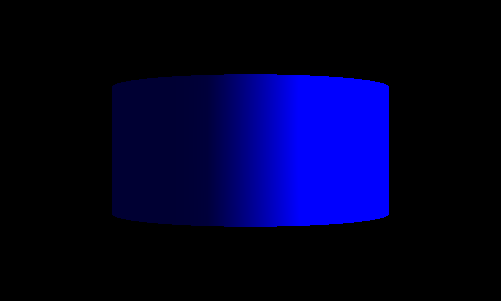
\includegraphics{primCylinder.png}
\caption{Cylinder.\label{fig:cylinder}}
\end{figure}

For image size, see:
\url{http://www.imagemagick.org/discourse-server/viewtopic.php?t=21076}

\subsubsection{Cone}\label{cone}

A cone aligned at the z-axis, with length 1, base cap, centered at the
origin, with radius $r_1 \in \mathbb{R}$, top cap, centered at
$\vec{p_2} = (0,0,1)$, with radius $r_2 \in \mathbb{R}$ is defined by
the set

\[
  \{\vec{p}=(x,y,z)| p \in \mathbb{R^3},
  \cos^2 \alpha * (x^2 + y^2) - \sin^2 \alpha * (z - r_1 / \alpha) = 0,
  1 \ge z \ge 0\}
\]

where the half-angle $\alpha = r_1 - r_2$

\section{Rendering}\label{rendering}

In the field of 3D computer graphics the process of generation a image
from a defined scene description is called rendering. Also the result of
this process is a rendering. In this section we shortly introduce
rasterization, because its the most used method for real time
applications. After that we introduce ray tracing and at the end of the
section we will compare both methods.

\hyperdef{}{rasterization}{\subsection{Rasterization}\label{rasterization}}

To render a scene with rasterization, we execute following steps:

\begin{itemize}
\itemsep1pt\parskip0pt\parsep0pt
\item
  Calculate the position, color and various attributes of the
  primitives.
\item
  Convert the primitives into fragments, which are stored in a raster
  image. This raster image stores location, color, depth and other
  informations.
\item
  Calculate the final color of each pixel based on the raster image.
\end{itemize}

For a introduction on this topic see \textbf{TODO add cite to the book:
https://www.ics.uci.edu/\textasciitilde{}gopi/CS211B/opengl\_programming\_guide\_8th\_edition.pdf}

\subsection{Ray Tracing}\label{ray-tracing}

Ray tracing is a rendering technique, which idea is to trace the path of
rays emitted from a camera that travel through pixels of a image. By
intersecting the rays with each object of a scene we can determine the
visible object for each ray. The visible object is the one with the
closest intersection. For each pixel corresponding to the ray we can
calculated the color with the properties(location, material, \ldots{})
of the closest object and the scene. These can implicate the generation
of new rays to simulate effects like reflection and refractions. There
are several ray tracing techniques that share the same basic algorithm.

\subsubsection{History}\label{history}

Some techniques for shading machine rederings of soilds is a paper of
Arthur Appel published in 1968 \cite{appel} it is the first approach to
ray tracing. He represented light rays as mathematical lines and checked
if there is a intersection with a object. After a intersection the light
rays aren't traced further, also known as Ray Casting. These process
doesn't considered shadows or reflections. \textbackslash{} Ray tracing
is a extension of Appels algorithm that was introduced by Whitted in
1980 \cite{whitt}. This extension considers shadow and reflections by
tracing rays/lines after the intersection. After a intersection a ray
can generate 3 new rays, the shadow ray, reflection ray and refraction
ray. These rays are called secondary rays. The starting point of a
shadow ray is the intersection point and its direction leads to a light
source. This is used to determine if the light source influences the
object at the intersection point. For example if a object is in between
the shadow ray and the light source the intersected point will not be
illuminated and will be represented as shadow. Reflection and refraction
rays are traced further, which makes the algorithm recursive.
\textbackslash{} Distribution ray tracing was introduced by Cook in 1984
\cite{cook}. This method increases realism of the image by using
probability distributions for specific effects and increases the number
of generated rays to approximate the result. For example generating
multiple shadow rays for area light sources to represent soft shadows.
Path tracing was introduces by Kajiya in 1986 \cite{kaji}. Applying
distributing rays not only to specific effects like shadows, but for the
shading of all diffuse surfaces. With these the illumination of the
lights with all object can be simulated correctly. This method is also
called monte carlo ray tracing, because it uses random samples to
compute the image.

\subsubsection{Basic Algorithm}\label{basic-algorithm}

The basic concept of a ray tracing algorithm is to find intersections of
a ray with a scene consisting of a set of geometric primitives
efficiently \cite{wald}. The ray, as defined in the section
\hyperref[ray]{Ray}, can have additional parameters $t_{min}$ and
$t_{max}$, which specifies the interval of $t$ used to define the set of
all points of the ray. In other words it specifies the minimum and the
maximum distance of a ray.

At this level the algorithm can be split in 3 tasks. The most
fundamental task is to find the closest intersection. The second task,
also called visibility/occlusion test, is to check if there are any
intersection of a ray with a object. The last task is find all
intersections of a ray. To check for any intersections is slightly
simpler as checking for the closest, so there are algorithms that are
more efficient in this case. For example the occlusion test is used for
shadow rays \cite{wald}. In ray tracing only one condition for a
primitive must apply, which is a be a function that can calculate a
intersection between the primitive and a ray. That means primitives can
be of various types, from simple geometric shapes like sphere, cubes,
trianles,\ldots{}, to complex parametric patches like the Bezier patches
and other complex shapes as long as there exist a intersection function.
The flexibility of primitives allows to represent shapes with full
accuracy. Although using multiple kinds of primitives does not limit the
kinds of scenes that can be rendered. Like mentioned in the section
\hyperref[rasterization]{Rasterization} most real time applications uses
rasterization techniques to render a image and most of them only uses
triangles as primitives.

Testing every primitive in the scene for a intersection with a ray
produce the correct result, but the computation time extends with each
ray and each primitives. For complex scenes it is necessary reduce the
set of primitives that the ray could intersect. To preserve consistency
its common to use acceleration data structures, e.g.~grids and kd-trees
\cite{copy}.

\subsubsection{Performance}\label{performance}

At the beginning of modern computer graphics only simple scenes were
used and interactive graphic applications weren't established. The
scenes didn't aim to be realistic. Ray tracing is computational intents
that aims to simulate realistic behavior. These are part of the reasons
why rasterization is the well-established rendering technique for
interactive applications and ray tracing is still seldom in this field.

However the demand of more detailed scenes, larger scenes and more
realism leads to the argument that ray tracing will outperform
rasterization at some point because of the logarithmic scene complexity
\cite{wald}.

Ray tracing is usually used for offline rendering due to the fact that
it is computational intents. The crucial factors for the ray tracing
algorithm are:

\begin{itemize}
\item
  The amount of rays. Consider a image with a resolution of 800 x 800
  and without counting the secondary rays. This results in a total
  amount of 640.000 rays. Considering the secondary rays the total
  number of rays would increase even further. Depending on the scene
  complexity the set of primary rays may only be small part compared to
  the set of all rays.
\item
  Scene complexity. Reducing the set of primitives for a ray with
  acceleration data structures is the most important optimization in ray
  tracing because it can give the algorithm a logarithmic behavior in
  scene complexity \cite{copy}.
\end{itemize}

The common crucial factors lead to common optimizations. For the first
fact, the amount of rays, its sufficed to reduce the number of rays to
reduce the computation time. This can be archived by reducing the
primary rays(smaller resolution) or reducing the secondary rays. The
second fact, the scene complexity, can be optimized by using the
mentioned acceleration data structures. Also using optimized
intersection functions leads to reduced computation time.
\textbackslash{} Ray tracing is knows as embarrassing parallel problem.
That means to execute the algorithm in parallel is trivial because the
result for each ray can be calculated independently. The optimization of
ray tracing is a topic of interest since the invention of the algorithm
\cite{copy}.

\subsection{Ray Tracing compared with
rasterization}\label{ray-tracing-compared-with-rasterization}

When compared to rasterization based rendering, ray tracing offers a
number of advantages. First of all, ray tracing is famous for the high
quality and realism of images that it can produce. This is why it is the
method of choice for offline rendering tasks where performance is not the
primary concern. Ray tracing is very flexible, as all rays can basically
be processed and shaded independently. This leads to simple and
intuitive implementations of even complex effects like shadows,
reflections and refractions. Using ray tracing, these effects are computed
correctly by default, whereas in rasterization based rendering this is
often not possible. Instead, a number of approximations (e.g.~shadow
maps, reflection cube maps, \ldots{}) must be used to simulate these
effects. This is often a non-trivial task and generating believable
results is usually only possible if the rendered scene meets certain
criteria. The flexibility of ray tracing makes it possible to use
approximations that are common in many applications using rasterization
based rendering. While it may involve some extra work, using them might
be desirable to achieve performance improvements. The key point here is
that ray tracing can use these approximations if required, but
rasterization based rendering is generally limited to using them and
therefore does not allow physically correct computation of many effects.

\section{Comments}\label{comments}

\begin{itemize}
\itemsep1pt\parskip0pt\parsep0pt
\item
  Give (mathematical) definitions
\item
  Use ``follows'' correctly
\item
  Use \texttt{git diff}!
\item
  Use uniform enumerations, e.g. ``translating, rotating, and scaling''
\item
  Give full definitions if possible, i.e.~do not ``truncate'' things
  afterwards
\item
  Refer to scientific papers
\item
  Use Markdown figures and refer to them in the text where appropriate
\item
  Sketch out structure before writing and refine
\end{itemize}

% END: content -------------------------------------------------------
\bibliographystyle{abbrv}
\bibliography{biblio}

\end{document}
